\documentclass[letterpaper,final,12pt,reqno]{amsart}

\usepackage[total={6.3in,9.2in},top=1.1in,left=1.1in]{geometry}

\usepackage{times,bm,bbm,empheq,verbatim,fancyvrb,graphicx}
\usepackage[dvipsnames]{xcolor}

\usepackage[kw]{pseudo}

\pseudoset{left-margin=15mm,topsep=5mm,idfont=\texttt}

\usepackage{tikz}
\usetikzlibrary{decorations.pathreplacing}

% hyperref should be the last package we load
\usepackage[pdftex,
colorlinks=true,
plainpages=false, % only if colorlinks=true
linkcolor=blue,   % ...
citecolor=Red,    % ...
urlcolor=black    % ...
]{hyperref}

\DefineVerbatimEnvironment{cline}{Verbatim}{fontsize=\small,xleftmargin=5mm}

\renewcommand{\baselinestretch}{1.05}

\newtheorem{lemma}{Lemma}

\newcommand{\Matlab}{\textsc{Matlab}\xspace}
\newcommand{\eps}{\epsilon}
\newcommand{\RR}{\mathbb{R}}

\newcommand{\grad}{\nabla}
\newcommand{\Div}{\nabla\cdot}
\newcommand{\trace}{\operatorname{tr}}

\newcommand{\hbn}{\hat{\mathbf{n}}}

\newcommand{\bb}{\mathbf{b}}
\newcommand{\be}{\mathbf{e}}
\newcommand{\bbf}{\mathbf{f}}
\newcommand{\bg}{\mathbf{g}}
\newcommand{\bn}{\mathbf{n}}
\newcommand{\br}{\mathbf{r}}
\newcommand{\bu}{\mathbf{u}}
\newcommand{\bv}{\mathbf{v}}
\newcommand{\bw}{\mathbf{w}}
\newcommand{\bx}{\mathbf{x}}

\newcommand{\bV}{\mathbf{V}}
\newcommand{\bX}{\mathbf{X}}

\newcommand{\bxi}{\bm{\xi}}

\newcommand{\bzero}{\bm{0}}

\newcommand{\rhoi}{\rho_{\text{i}}}
\newcommand{\ip}[2]{\left<#1,#2\right>}

\newcommand{\Rpr}{R_{\text{pr}}}
\newcommand{\Rin}{R_{\text{in}}}
\newcommand{\Rfw}{R_{\text{fw}}}


\begin{document}
\title[The FAS multigrid scheme]{The full approximation storage multigrid scheme: \\ A 1D finite element example}

\author{Ed Bueler}

\begin{abstract}  This note describes the full approximation storage (FAS) multigrid scheme for an easy one-dimensional nonlinear boundary value problem.  The problem is discretized by a simple finite element (FE) scheme.  We apply both FAS V-cycles and F-cycles, with a nonlinear Gauss-Seidel smoother, to solve the resulting finite-dimensional problem.  The mathematics of the FAS restriction and prolongation operators, in the FE case, are explained.  A self-contained Python program implements the scheme.  Optimal performance, i.e.~work proportional to the number of unknowns, is demonstrated for both kinds of cycles, including convergence nearly to discretization error in a single F-cycle.  \end{abstract}

\thanks{Version 2.  This note is expository and submission for publication is not foreseen.}

\maketitle

\tableofcontents

\thispagestyle{empty}
\bigskip

\section{Introduction}  \label{sec:intro}

We consider the full approximation storage (FAS) scheme, originally described by Brandt \cite{Brandt1977}, for an easy nonlinear elliptic equation.  Like other multigrid schemes it exhibits optimal solver complexity \cite{Bueler2021} when correctly applied, as we demonstrate at the end.  Helpful write-ups of FAS can be found in well-known textbooks \cite{BrandtLivne2011,Briggsetal2000,Trottenbergetal2001}, but we describe the scheme from a finite element point of view, compatible with the multigrid approaches used for obstacle problems \cite{GraeserKornhuber2009} for example, and we provide an easy-to-digest Python implementation.

Our problem is an ordinary differential equation (ODE) boundary value problem, the nonlinear Liouville-Bratu equation \cite{Bratu1914,Liouville1853}:
\begin{equation}
  -u'' - \lambda\, e^u = g,  \qquad u(0) = u(1) = 0.  \label{liouvillebratu}
\end{equation}
In this problem $\lambda$ is a real constant, $g(x)$ is given, and we seek $u(x)$.  This equation arises in the theory of combustion \cite{FrankKameneckij1955} and the stability of stars.

Our goal is to solve \eqref{liouvillebratu} in optimal $O(m)$ time on a mesh of $m$ elements.  A Python implementation of FAS, \texttt{fas1.py} in directory \texttt{fas/py/},\footnote{Clone the Git repository\, \href{https://github.com/bueler/mg-glaciers}{\texttt{github.com/bueler/mg-glaciers}}\, and look in the \texttt{fas/py/} directory.} accomplishes such optimal-time solutions both by V-cycle and F-cycle strategies (section \ref{sec:cycles}).  (This note serves as its documentation.)  While optimal-time solutions of 1D problems are not unusual, FAS and other multigrid strategies for many nonlinear 2D and 3D partial differential equations (PDEs) are also optimal.  This makes them the highest-performing class of solver algorithms for such problems.

By default the program \texttt{fas1.py} solves \eqref{liouvillebratu} with $g=0$.  A runtime option \texttt{-mms}, the ``method of manufactured solutions'' \cite{Bueler2021}, facilitates testing by specifying a problem with known exact solution and nonzero source term.  In detail, the solution is $u(x)=\sin(3\pi x)$, and by differentiation $g(x)=9\pi^2 \sin(3\pi x) - \lambda e^{\sin(3\pi x)}$.


\section{The finite element method}  \label{sec:femethod}

To solve the problem using the finite element (FE) method \cite{Braess2007,Bueler2021,Elmanetal2014}, we rewrite \eqref{liouvillebratu} in weak form.  Let $F$ be the nonlinear operator
\begin{equation}
  F(u)[v] = \int_0^1 u'(x) v'(x) - \lambda e^{u(x)} v(x)\, dx,  \label{operator}
\end{equation}
acting on $u$ and $v$ from the space of functions $\mathcal{H}=H_0^1[0,1]$, a Sobolev space \cite{Evans2010}.  (These functions have zero boundary values and one square-integrable derivative.)  Note $F(u)[v]$ is linear in $v$ but not in $u$.  We also define a linear functional from the right-hand function $g$ in \eqref{liouvillebratu}:
\begin{equation}
  \ell[v] = \ip{g}{v} = \int_0^1 g(x) v(x) dx.  \label{rhsfunctional}
\end{equation}
Both $F(u)[\cdot]$ and $\ell[\cdot]$ are (continuous) linear functionals, acting on functions $v$ in $\mathcal{H}$, thus they are in the dual space $\mathcal{H}'$.  One derives the weak form
\begin{equation}
  F(u)[v] = \ell[v] \qquad \text{for all $v$ in $\mathcal{H}$} \label{weakform}
\end{equation}
by multiplying equation \eqref{liouvillebratu} by a test function $v$ and integrating by parts.

From now on we address problem \eqref{weakform}, despite its abstract form.  In an FE context a clear separation is desirable between functions, like the solution $u(x)$, and the equations themselves, which are, essentially, functionals.  As in linear algebra, where one indexes the equations by row indices, \eqref{weakform} states ``$v$th equation''; the equations are indexed by the test functions.  The FE method will reduce the problem to a finite number of unknowns by writing $u(x)$ in a basis of a finite-dimensional subspace of $\mathcal{H}$.  One gets finitely-many equations by using test functions $v$ from the same basis.

We apply the simplest possible mesh setup, namely an equally-spaced mesh on $[0,1]$ of $m$ elements (subintervals) of lengths $h=1/m$.  The interior nodes (points) are $x_p=ph$ for $p=1,\dots,m-1$.  This mesh supports a finite-dimensional vector subspace of $\mathcal{H}$:
\begin{equation}
\mathcal{S}^h = \left\{v(x)\,\big|\,v \text{ is continuous, linear on each subinterval, and } v(0)=v(1)=0\right\}.  \label{fespace}
\end{equation}
This space has a basis of ``hat'' functions $\{\psi_p(x)\}$, one for each interior node (Figure \ref{fig:onehat}).  Such a hat function $\psi_p$ is defined by two properties: $\psi_p$ is in $\mathcal{S}^h$ and $\psi_p(x_q)=\delta_{pq}$ for all $q$.  Note that the $L^2$ norm of $\psi_p$ depends on the mesh resolution $h$, and that $\ip{\psi_p}{\psi_q}\ne 0$ for only three indices $q=p-1,p,p+1$.  The basis of hat functions, while well-conditioned, is not orthonormal.

\begin{figure}
\includegraphics[width=0.6\textwidth]{figs/onehat.pdf}
\caption{A piecewise-linear hat function $\psi_p(x)$ lives at each interior node $x_p$.}
\label{fig:onehat}
\end{figure}

The numerical solution $u^h$ has the expansion
\begin{equation}
  u^h(x) = \sum_{p=1}^{m-1} u[p] \psi_p(x)  \label{fesolution}
\end{equation}
with coefficients $u[p]$ equal to the point values $u^h(x_p)$.  That is, because the hat functions form a ``nodal basis'' \cite{Elmanetal2014}, $u^h$ may be represented as a vector $\bu$ in $\RR^{m-1}$ either by its coefficients in the basis $\{\psi_p\}$ or its point values:
\begin{equation}
\bu =\{u[p]\} = \{u^h(x_p)\}.  \label{fevector}
\end{equation}

The FE approximation $F^h$ of the nonlinear operator $F$ in \eqref{operator} acts on functions in $\mathcal{S}^h$.  Its values $F^h(w^h)[\psi_p]$ are easily computed if the transcendental integral is approximated, for example by using the trapezoid rule, as follows.  Noting that the support of $\psi_p(x)$ is $[x_{p-1},x_{p+1}]$, and that the derivative of $\psi_p$ is $\pm 1/h$, we have:
\begin{align}
  F(w^h)[\psi_p] &= \int_0^1 (w^h)'(x) \psi_p'(x) - \lambda e^{w^h(x)} \psi_p(x)\, dx  \label{feoperator} \\
    &= \int_{x_{p-1}}^{x_{p+1}} (w^h)'(x) (\pm 1/h)\,dx - \lambda \int_{x_{p-1}}^{x_{p+1}} e^{w^h(x)} \psi_p(x)\, dx \notag \\
    &\approx h \left(\frac{w[p]-w[p-1]}{h} - \frac{w[p+1]-w[p]}{h}\right) - h \lambda e^{w[p]}  \notag \\
    &= \frac{1}{h}\left(2w[p]-w[p-1]-w[p+1]\right) - h \lambda e^{w[p]} \notag \\
    &= F^h(w^h)[\psi_p] \notag
\end{align}
Note that $F^h$ is a rescaled version of a well-known $O(h^2)$ finite difference expression.  Function \texttt{FF()} in \texttt{fas1.py} computes this formula.

Now consider the right-hand-side functional $\ell[v]$ in \eqref{weakform}, which we will approximate by $\ell^h[v]$ acting on $\mathcal{S}^h$.  We again apply the trapezoid rule to compute the integral $\ip{g}{\psi_p}$, and we get the simple formula
\begin{equation}
  \ell^h[\psi_p] = h\, g(x_p). \label{ferhs}
\end{equation}
The linear functional $\ell^h$ and the function $g$ are different objects, though they only differ by a factor of the mesh size $h$.

The finite element weak form can now be stated:
\begin{equation}
  F^h(u^h)[v] = \ell^h[v] \qquad \text{for all } v \text{ in } \mathcal{S}^h. \label{feweakform}
\end{equation}
To solve \eqref{feweakform} we seek an iterate $w^h$ so that the \emph{residual}
\begin{equation}
  r^h(w^h)[v] = \ell^h[v] - F^h(w^h)[v]  \label{feresidual}
\end{equation}
is small for all $v$ in $\mathcal{S}^h$.  Again $r^h(w^h)$ is a linear functional acting on functions in $\mathcal{S}_h$, so it suffices to apply it to a basis of test functions $v=\psi_p$:
\begin{equation}
  r^h(w^h)[\psi_p] = \ell^h[\psi_p] - \frac{1}{h}\left(2w[p]-w[p-1]-w[p+1]\right) + h \lambda e^{w[p]}.  \label{feresidualdetail}
\end{equation}
Solving the finite-dimensional nonlinear system, i.e.~the FE approximation of \eqref{weakform}, is equivalent to finding $w^h$ in $\mathcal{S}^h$ so that $r^h(w^h)[\psi_p]=0$ for $p=1,\dots,m-1$.

A function in \texttt{fas1.py} computes \eqref{feresidualdetail} for any source functional $\ell^h$.  On the original mesh, soon to be called the ``fine mesh'', we will use formula \eqref{ferhs}.  However, the FAS algorithm (sections \ref{sec:fastwolevel} and \ref{sec:cycles}) is a systematic way to introduce a new source functional on each coarser mesh.

The function $u^h(x)$ in $\mathcal{S}^h$, equivalently $\bu$ in $\RR^{m-1}$ given by \eqref{fevector}, exactly solves a finite-dimensional nonlinear system \eqref{feweakform}.  In practice, however, at each stage we only possess an iterate $w^h(x)$, for which the ``algebraic error'' is
\begin{equation}
  e^h = w^h - u^h.  \label{feerror}
\end{equation}
On the other hand, $u^h$ is not the continuum solution either; the ``discretization error'' $u^h-u$, where $u$ is the exact solution of the continuum problem \eqref{weakform}, is also nonzero in general.  The theory of an FE method will show that discretization error goes to zero as $h\to 0$, at a particular rate determined by the FE space and the smoothness of the continuum problem \cite{Elmanetal2014}, but such a theory assumes we have exactly-solved the finite-dimensional system, i.e.~that we possess $u^h$ itself.  The full ``numerical error'' is the difference $w^h-u$, and we have
\begin{equation}
\|w^h-u\| \le \|w^h-u^h\|+\|u^h-u\|.
\end{equation}
The numerical error, which we want to control, is bounded by the algebraic error plus the discretization error.

In the \texttt{-mms} case of \texttt{fas1.py}, where the exact solution $u$ of the continuum problem is known, the numerical error norm $\|w^h-u\|$ is computable.  Normally we cannot access $u$ or $u^h$ directly, and only the residual norm $\|r^h(w^h)\|$ is computable, but the numerical error is controlled to within a matrix condition number by the residual norm.


\section{The nonlinear Gauss-Seidel iteration}  \label{sec:ngs}

Next we describe an iteration which will, if carried far enough, solve the finite-dimensional nonlinear system \eqref{feweakform} to desired accuracy.  This is the nonlinear Gauss-Seidel (NGS) iteration \cite{Briggsetal2000}, also called Gauss-Seidel-Newton \cite{BrandtLivne2011}.  It updates the iterate $w^h$ by changing each point value at $x_p$ to make the residual at that point zero.  That is, NGS solves the problem
\begin{equation}
\phi(c) = r^h(w^h + c \psi_p)[\psi_p] = 0  \label{ngspointproblem}
\end{equation}
for a scalar $c$.  Once $c$ is found we update the point value (coefficient):
\begin{equation}
  w^h \leftarrow w^h + c \psi_p,  \label{ngspointupdate}
\end{equation}
equivalently $w[p] \leftarrow w[p] + c$.

As in the linear Gauss-Seidel iteration \cite{Greenbaum1997}, $w[p]$ is updated in a certain nodal ordering, using current values $w[q]$ when evaluating the residual in \eqref{ngspointproblem}.  However, as the residual is made zero at one point it is no longer zero at the previous points.  Gauss-Seidel-type methods are called ``successive'' \cite{GraeserKornhuber2009} or ``multiplicative'' \cite{Bueler2021} corrections.  ``Additive'' corrections, of which the Jacobi iteration \cite{Greenbaum1997} is the best known, are also possible, but they are somewhat less efficient.  Note our program only runs in serial, so the parallelizability of the Jacobi iteration cannot be exploited.

Solving the scalar problem $\phi(c)=0$ cannot be done exactly when considering a transcendental problem like \eqref{liouvillebratu}.  Instead we will use a fixed number of Newton iterations \cite[Chapter 4]{Bueler2021} to generate a (scalar) sequence $\{c_k\}$ converging to $c$.  Starting from $c_0=0$ we compute
\begin{equation}
\phi'(c_k)\, s_k = -\phi(c_k),  \qquad  c_{k+1} = c_k + s_k, \label{ngsnewton}
\end{equation}
for $k=0,1,\dots$.  From \eqref{feresidualdetail} we have
\begin{align*}
 \phi(c) &= \ell^h[\psi_p] - \frac{1}{h} \left(2(w[p]+c) - w[p-1] - w[p+1]\right) + h \lambda e^{w[p]+c}, \\
\phi'(c) &= -\frac{2}{h} + h \lambda e^{w[p]+c}.
\end{align*}
The vast majority of the work of our FAS algorithms will be in evaluating these expressions.

The NGS method ``sweeps'' through the mesh, zeroing $\phi(c)$ at successive nodes $x_p$, in increasing $p$ order, as in the following pseudocode which modifies $w^h$ in-place:
\begin{pseudo*}
\pr{ngssweep}(w^h,\ell^h,\id{niters}=2)\text{:} \\+
    $r(w^h)[v] := \ell^h[v] - F^h(w^h)[v]$ \\
    for $p=1,\dots,m-1$ \\+
        $\phi(c) := r^h(w^h + c \psi_p)[\psi_p]$ \\
        $c=0$ \\
        for $k=1,\dots,$\id{niters} \\+
            $c \gets c - \phi(c) / \phi'(c)$ \\-
        $w[p] \gets w[p] + c$
\end{pseudo*}
For FAS algorithms (next section) we also define \textsc{ngssweep-back} with ``\textbf{for} $p=m-1,\dots,1$''.  Function \texttt{ngssweep()} in \texttt{fas1.py} computes either order, and the \texttt{niters} default is two.

For a linear differential equation the Gauss-Seidel iteration is known to converge subject to matrix assumptions which correspond to ellipticity of the original problem \cite[for example]{Greenbaum1997}.  We expect that for weak nonlinearities, e.g.~small $\lambda$ in \eqref{liouvillebratu}, our method will therefore converge as a solution method for \eqref{feweakform}, and we will demonstrate that this occurs in practice (section \ref{sec:convergence}).  However, one observes in practice that, after substantial progress in the first few sweeps during which the residual becomes very smooth, soon NGS stagnates.  Following Brandt \cite{Brandt1977,BrandtLivne2011}, who asserts that such a stalling scheme must be ``wrong'', we adopt the multigrid approach next.


\section{The FAS equation for two levels}  \label{sec:fastwolevel}

The fundamental goal of any multigrid scheme is to do a minimal amount of work (smoothing) on a given mesh and then to switch to an inexpensive coarser mesh to do the rest of the work.  By transferring (restricting) a version of the problem to the coarser mesh one can nearly solve for the error.  The coarse-mesh approximation of the error is then added-back (prolonged) to correct the solution on the finer mesh.  Being a multigrid scheme, full approximation storage (FAS) \cite{Brandt1977,Briggsetal2000} must therefore include the following elements:
\renewcommand{\labelenumi}{(\roman{enumi})}
\begin{enumerate}
\item a hierarchy of meshes, with restriction and prolongation operators between levels,
\item a ``smoother'' for each level, and
\item a meaningful way to transfer the problem to a coarser mesh.
\end{enumerate}

Regarding (i), we describe only two levels at first, but a full mesh hierarchy is used in section \ref{sec:cycles}.  Here our coarse mesh has spacing $2h$ and $m/2$ elements (subintervals); all quantities on the coarse mesh have superscript ``$2h$''.  The program \texttt{fas1.py} only refines by factors of two, but the ideas generalize for other refinement factors.

For (ii), a small fixed number of NGS sweeps is our smoother on the fine mesh.  Each sweep, given by algorithm \textsc{ngssweep} above, is an $O(m)$ operation with a small constant.  (The constant is determined by the number of Newton iterations and the expense of evaluating nonlinearities at each point, e.g.~$\lambda e^u$ in \eqref{liouvillebratu}.)  A few NGS sweeps produces the results that the fine-mesh residual $r^h(w^h)$ and algebraic error $e^h = w^h - u^h$ becomee smooth, but they do not necessarily become small.  Using more sweeps of NGS would eventually make the error small, and solve problem \eqref{feweakform}, but inefficiently in the sense that many sweeps would be needed, generally giving an $O(m^q)$ method for $q\gg 1$.  However, NGS sweeps on a coarser mesh will see the coarse-mesh interpolant of the fine-mesh residual as less smooth, so the coarser-mesh NGS can quickly eliminate a large fraction of the error.  Descending to yet coarser meshes, in a V-cycle as described in section \ref{sec:cycles}, leads to a coarsest mesh on which the error can be eliminated entirely by applying NGS at only a few interior points.  (In the default settings for \texttt{fas1.py}, the coarsest mesh has two subintervals and one interior point.)

For item (iii), what is the coarse-mesh version of the problem?  To derive this equation, namely to explain Brandt's FAS equation \cite{Brandt1977}, we start from the FE weak form \eqref{feweakform}.  The fine-mesh solution $u^h$ is generally unknown.  For an iterate $w^h$ we subtract $F^h(w^h)[v]$ from both sides to get the residual \eqref{feresidual} on the right:
\begin{equation}
  F^h(u^h)[v] - F^h(w^h)[v] = r^h(w^h)[v]. \label{fasproto}
\end{equation}
It is not yet the FAS equation, but three key observations apply to equation \eqref{fasproto}:
\begin{itemize}
\item Both $w^h$ and $r^h(w^h)$ are known and/or computable.
\item If NGS sweeps have been applied to $w^h$ then $e^h=w^h-u^h$ and $r^h(w^h)$ are smooth.
\item If $F^h$ were linear in $w^h$ then we could rewrite the equation in terms of the error:
    $$\qquad\qquad\qquad\qquad F^h(e^h)[v] = -r^h(w^h)[v] \qquad\qquad (\text{\emph{if $F^h$ is linear}}).$$
(One could even write the error equation using a matrix, i.e.~$A\be=-\br$.)
\end{itemize}

Based on these observations, Brandt proposed proposed a new nonlinear equation on the coarse mesh.  It is derived from \eqref{fasproto} by replacing terms using restriction operators on the computable quantities and by re-discretizing the nonlinear operator to get $F^{2h}$ acting on $\mathcal{S}^{2h}$.  Because the problem is nonlinear we must store a coarse-mesh approximation   to the solution, namely $u^{2h}$ in $\mathcal{S}^{2h}$, not just the error.  Denoting the restriction operators by $R'$ and $R$, which are addressed in the next section, the following is the FAS equation:
\begin{equation}
  F^{2h}(u^{2h})[v] - F^{2h}(R w^h)[v] = R' (r^h(w^h))[v], \label{faspreequation}
\end{equation}
for all $v$ in $\mathcal{S}^{2h}$.  We can simplify the appearance by trivial rearrangement,
\begin{equation}
  F^{2h}(u^{2h})[v] = \ell^h[v], \label{fasequation}
\end{equation}
where
\begin{equation}
  \ell^{2h}[v] = R' (r^h(w^h))[v] + F^{2h}(R w^h)[v]. \label{fasell}
\end{equation}

The key idea behind the FAS equation \eqref{fasequation}, which has the same form as the fine-mesh weak form \eqref{feweakform}, is that the smoothness of the error and residual have allowed us to accurately transfer the problem to the coarser mesh.  Note that if $w^h=u^h$, that is, if $w^h$ is the exact solution to the fine-mesh problem \eqref{feweakform}, then $r^h(w^h)=0$ so $\ell^{2h}$ simplifies to $F^{2h}(R w^h)[v]$, and the solution of \eqref{fasequation} would be $u^{2h} = R w^h$ by well-posedness.

Next, in stating the two-level FAS method we will suppose \eqref{fasequation} is solved exactly, so $u^{2h}$ and the coarse-mesh error $u^{2h}-Rw^h$ are known.  We will update the iterate on the finer mesh by adding a fine-mesh version the error:
\begin{equation}
  w^h \gets w^h + P(u^{2h} - R w^h) \label{fasupdate}
\end{equation}
Here $P$ is a prolongation operator (next section); it extends a function in $\mathcal{S}^{2h}$ to a function in $\mathcal{S}^h$.  Supposing that the smoother and the restriction/prolongation operators $R',R,P$ are all determined, formulas \eqref{fasequation}, \eqref{fasell}, and \eqref{fasupdate} define the following in-place algorithm in which $F^h$ and $F^{2h}$ denote discretizations of $F$ on the two meshes:
\label{fastwolevel}
\begin{pseudo*}
\pr{fas-twolevel}(w^h,\ell^h,\id{down}=1,\id{up}=1)\text{:} \\+
    for $j=1,\dots,$\id{down} \\+
        \pr{ngssweep}(w^h,\ell^h) \\-
    $\ell^{2h}[v] := R' (\ell^h-F^h(w^h))[v] + F^{2h}(R w^h)[v]$ \\
    $w^{2h} = \pr{copy}(R w^h)$ \\
    \pr{coarsesolve}(w^{2h},\ell^{2h}) \\
    $w^h \gets w^h + P(w^{2h} - R w^h)$ \\
    for $j=1,\dots,$\id{up} \\+
        \pr{ngssweep-back}(w^h,\ell^h)
\end{pseudo*}
We allow smoothing before and after the coarse-mesh correction.  Specifically, \texttt{down} forward NGS sweeps modify $w^h$ before the coarse-mesh correction and \texttt{up} backward sweeps after.

While it is common in linear multigrid \cite{Briggsetal2000,Bueler2021,Trottenbergetal2001} to apply a direct solver like LU decomposition as the coarse-mesh solver, our problem is nonlinear so no finite-time direct solver is available.  Instead we do enough NGS sweeps to solve the coarse-mesh problem accurately:
\begin{pseudo*}
\pr{coarsesolve}(w,\ell,\id{coarse}=1)\text{:} \\+
    for $j=1,\dots,$\id{coarse} \\+
        \pr{ngssweep}(w,\ell)
\end{pseudo*}

In order to implement FAS we must define the action of operators $R'$, $R$, and $P$ in \eqref{fasell} and \eqref{fasupdate},which is done next.  In section \ref{sec:cycles} we will define an FAS V-cycle by replacing \textsc{coarsesolve} with the recursive application of the FAS solver itself.


\section{Restriction and prolongation operators} \label{sec:restrictionprolongation}

To explain the two different restriction operators $R'$ and $R$ in \eqref{fasequation}, plus the prolongation $P$ in \eqref{fasupdate}, first note that functions $w^h$ in $\mathcal{S}^h$ are distinct objects from linear functionals like the residual $r^h(w^h)$.  Denoting such linear functionals by $(\mathcal{S}^h)'$, the three operators are already distinguished by their domain and range spaces:
\begin{align}
  R' &: (\mathcal{S}^h)' \to (\mathcal{S}^{2h})', \label{rpoperators} \\
  R  &: \mathcal{S}^h \to \mathcal{S}^{2h}, \notag \\
  P  &: \mathcal{S}^{2h} \to \mathcal{S}^h. \notag
\end{align}

On the other hand, both functions in $\mathcal{S}^h$ and linear functionals in $(\mathcal{S}^h)'$ are representable by vectors in $\RR^{m-1}$.  One stores a function $w^h$ via coefficients $w[p]$ with respect to an expansion in the hat function basis $\{\psi_p\}$, as in \eqref{fesolution} for example, while one stores a functional $\ell^h$ by its values $\ell^h[\psi_p]$.  Though it makes sense to represent $w^h$ as a column vector and $\ell^h$ as a row vector \cite{TrefethenBau1997}, in Python one may use ``flat'' one-dimensional NumPy arrays for both purposes.  For our problem an iterate $w^h$ has zero boundary values, and likewise $\ell^h$ acts on $v$ with zero boundary values, thus only interior-point hat functions are needed in these representations.

But how do $R'$, $R$, and $P$ actually operate in the finite element (FE) case?  The key calculation relates the coarse-mesh hat functions $\psi_q^{2h}(x)$ to the fine mesh hats $\psi_p^h(x)$ (Figure \ref{fig:hatcombination}):
\begin{equation}
  \psi_q^{2h}(x) = \frac{1}{2} \psi_{2q-1}^h(x) + \psi_{2q}^h(x) + \frac{1}{2} \psi_{2q+1}^h(x), \label{hatrelation}
\end{equation}
for $q=1,2,\dots,M-1$.  Recall that $M=m/2$, and that we are assuming $m$ is even.

\begin{figure}
\includegraphics[width=0.6\textwidth]{figs/hatcombination.pdf}
\caption{Formula \eqref{hatrelation} writes a coarse-mesh hat $\psi_q^{2h}(x)$ (solid) as a linear combination of fine-mesh hats $\psi_p^h(x)$ (dotted) for $p=2q-1,2q,2q+1$.}
\label{fig:hatcombination}
\end{figure}

First consider the prolongation $P$.  Because a piecewise-linear function on the coarse mesh is also a piecewise-linear function on the fine mesh, $P$ is defined as the injection of $\mathcal{S}^{2h}$ into $\mathcal{S}^h$, without changing the function.  Suppose $w^{2h}(x)$ is in $\mathcal{S}^{2h}$, so $w^{2h}(x) = \sum_{q=1}^{M-1} w[q] \psi_q^{2h}(x)$.  Then we use \eqref{hatrelation} to compute $P w^{2h}$ in terms of fine-mesh hat functions:
\begin{align}
(P w^{2h})(x) &= \sum_{q=1}^{M-1} w[q] \left(\frac{1}{2} \psi_{2q-1}^h(x) + \psi_{2q}^h(x) + \frac{1}{2} \psi_{2q+1}^h(x)\right) \label{pformula} \\
              &= \frac{1}{2} w[1] \psi_1^h(x) + w[1] \psi_2^h(x) + \left(\frac{1}{2} w[1] + \frac{1}{2} w[2]\right) \psi_3^h(x) + w[2] \psi_4^h(x) \notag \\
              &\qquad + \left(\frac{1}{2} w[2] + \frac{1}{2} w[3]\right) \psi_5^h(x) + \dots + w[M\!-\!1] \psi_{m-2}^h(x) \notag \\
              &\qquad + \frac{1}{2} w[M\!-\!1] \psi_{m-1}^h(x) \notag
\end{align}
As a matrix, $P:\RR^{M-1} \to \RR^{m-1}$ acts on vectors; it has $M-1$ columns and $m-1$ rows:
\begin{equation}
P = \begin{bmatrix}
1/2 & & & \\
1 & & & \\
1/2 & 1/2 & & \\
 & 1 & & \\
 & 1/2 & 1/2 & \\
 & & & \ddots
\end{bmatrix} \label{pmatrix}
\end{equation}
The columns of $P$ are linearly-independent and the column sums equal two by \eqref{hatrelation}.  The row sums equal one except for the first and last rows.

Next, the restriction $R'$ acts on fine-mesh linear functionals $\ell:\mathcal{S}^h \to \RR$.  It is called ``canonical restriction'' \cite{GraeserKornhuber2009} because its output, the functional $R'\ell:\mathcal{S}^{2h}\to \RR$, acts on coarse-mesh functions the same way as $\ell$ itself acts on those functions, so defining $R'$ involves no choices.  We may state this using $P$:
\begin{equation}
  (R'\ell)[v] = \ell[Pv],  \label{rprimedefinition}
\end{equation}
for $v$ in $\mathcal{S}^{2h}$.  As noted earlier, $\ell$ is represented by a vector in $\RR^{m-1}$ of the values $\ell[\psi_p^h]$, so one computes the values of $R'\ell$ using \eqref{hatrelation}:
\begin{align}
  (R'\ell)[\psi_q^{2h}] &= \ell[\psi_q^{2h}] = \ell\left[\frac{1}{2} \psi_{2q-1}^h + \psi_{2q}^h + \frac{1}{2} \psi_{2q+1}^h\right]  \label{rprimeformula} \\
      &= \frac{1}{2} \ell[\psi_{2q-1}^h] + \ell[\psi_{2q}^h] + \frac{1}{2} \ell[\psi_{2q+1}^h].  \notag
\end{align}
As a matrix $R'$ is the matrix transpose of $P$, with $M-1$ rows and $m-1$ columns:
\begin{equation}
R' = \begin{bmatrix}
1/2 & 1 & 1/2 &   &     & \\
    &   & 1/2 & 1 & 1/2 & \\
    &   &     &   & 1/2 & \\
    &   &     &   &     & \ddots
\end{bmatrix} \label{rprimematrix}
\end{equation}

Finally we consider the restriction $R:\mathcal{S}^h\to\mathcal{S}^{2h}$ acting on functions, a more interesting map because it loses information.  (By contrast, $P$ and $R'$ essentially preserve the input object, without loss, via reinterpretation on the output mesh.)  Consider a fine-mesh function $w^h = \sum_{p=1}^{m-1} w[p] \psi_p^{h}$.  The result $R w^h$ is linear across those fine-mesh nodes which are not in the coarse mesh, and so the values at those in-between nodes are not recoverable.

There are three well-known versions of the restriction $R$:
\begin{itemize}
\item $\Rpr$ is defined as projection, by the property
\begin{equation}
  \ip{\Rpr w^h}{v} = \ip{w^h}{v} \label{rprdefinition}
\end{equation}
for all $v\in \mathcal{S}^{2h}$.  Computing the entries of $\Rpr$ requires solving a linear system.  To show this system we define the invertible, sparse, symmetric mass matrices \cite{Elmanetal2014}, namely $Q_{jk}^{h} = \ip{\psi_j^{h}}{\psi_k^{h}}$ for the fine mesh and $Q_{jk}^{2h} = \ip{\psi_j^{2h}}{\psi_k^{2h}}$ for the coarse.  Then one solves a matrix equation for $\Rpr$:
\begin{equation}
  Q^{2h} \Rpr = R' Q^{h},  \label{rprequation}
\end{equation}
or equivalently $\Rpr = (Q^{2h})^{-1} R' Q^{h}$.  Equation \eqref{rprequation} is justified by using $v=\psi_s^{2h}$ in definition \eqref{rprdefinition}, and then applying \eqref{hatrelation}, as follows.  Write $z = \Rpr w^h = \sum_{q=1}^{M-1} z[q] \psi_q^{2h}$ and expand both sides:
\begin{align*}
\ip{z}{\psi_s^{2h}} &= \ip{w^h}{\psi_s^{2h}} \\
\sum_{q=1}^{M-1} z[q] \ip{\psi_q^{2h}}{\psi_s^{2h}} &= \sum_{p=1}^{m-1} w[p] \ip{\psi_p^{h}}{\frac{1}{2} \psi_{2s-1}^{h} + \psi_{2s}^{h} + \frac{1}{2} \psi_{2s+1}^{h}} \\
\sum_{q=1}^{M-1} Q_{sq}^{2h} z[q] &= \sum_{p=1}^{m-1} \left(\frac{1}{2} Q_{2s-1,p} + Q_{2s,p} + \frac{1}{2} Q_{2s+1,p}\right) w[p] \\
(Q^{2h} \Rpr w^h)[s] &= (R' Q^h w^h)[s]
\end{align*}
(Note $w^h$ in $\mathcal{S}^h$ and index $s$ are arbitrary.)  In 1D the mass matrices $Q^{2h},Q^h$ are tridiagonal, thus each column of $\Rpr$ can be found by solving equation \eqref{rprequation} using an $O(M)$ algorithm \cite{TrefethenBau1997}, implying $O(M^2)$ work.  While this is possible, and the result could even be found by hand in this case, the alternatives below are easier to implement.
\item $\Rin$ is defined as pointwise injection.  Supposing $w^h = \sum_{p=1}^{m-1} w[p] \psi_p^{h}$,
\begin{equation}
  \Rin w^h = \sum_{q=1}^{M-1} w[2q] \psi_q^{2h}, \label{rindefinition}
\end{equation}
so $(\Rin w^h)(x_q) = w^h(x_q) = w[2q]$ for each point $x_q$.  In other words, to compute $\Rin w^h$ we simply drop the nodal values at those fine-mesh nodes which are not in the coarse mesh.  As a matrix this is
\begin{equation}
\Rin = \begin{bmatrix}
0 & 1 &   &   &   &   &\\
  &   & 0 & 1 &   &   & \\
  &   &   &   & 0 & 1 & \\
  &   &   &   &   &   & \ddots
\end{bmatrix}. \label{rinmatrix}
\end{equation}
This restriction is very simple but it may lose track of the magnitude of $w^h$, or badly mis-represent it, \emph{if} the input is not smooth.  For example, sampling a sawtooth function at the coarse-mesh nodes would capture only the peaks or only the troughs.
\item $\Rfw$, the ``full-weighting'' restriction \cite{Briggsetal2000}, averages nodal values onto the coarse mesh:
\begin{equation}
  \Rfw w^h = \sum_{q=1}^{M-1} \left(\frac{1}{4} w[2q-1] + \frac{1}{2} w[2q] + \frac{1}{4} w[2q+1]\right) \psi_q^{2h}. \label{rfwdefinition}
\end{equation}
This computes each coarse-mesh nodal value of $z=\Rfw w^h$ as a weighted average of the value of $w^h$ at the three closest fine-mesh nodes.  The matrix is thus a multiple of the canonical restriction matrix in \eqref{rprimematrix}:
\begin{equation}
\Rfw = \begin{bmatrix}
1/4 & 1/2 & 1/4 &     &     &  \\
    &     & 1/4 & 1/2 & 1/4 &  \\
    &     &     &     & 1/4 &  \\
    &     &     &     &     & \ddots
\end{bmatrix} = \frac{1}{2} R'. \label{rfwmatrix}
\end{equation}
\end{itemize}

\medskip
Which restriction do we choose?  Because of their simplicity, we will implement and compare $\Rfw$ and $\Rin$ in \texttt{fas1.py}.


\section{Cycles} \label{sec:cycles}

The main principles of the FAS scheme are already contained in the \textsc{fas-twolevel} algorithm in section \ref{sec:fastwolevel}, from which it is a small step to solve the coarse-mesh problem by the same scheme, creating a so-called ``V-cycle''.  To define this precisely we need an indexed hierarchy of mesh levels.  Start with a coarsest mesh with $m_0$ elements of length $h_0=1/m_0$.  (By default in \texttt{fas1.py} we have $m_0=2$.)  For $k=1,\dots,K$ we refine by factors of two so that the $k$th mesh has $m_k=2^k m_0$ elements of length $h_k=h_0/2^k$.  The final $K$th mesh is now called the ``fine mesh''.  Instead of the superscripts $h$ and $2h$ used in section \ref{sec:fastwolevel}, now we use a ``$k$'' superscript to indicate the mesh on which a quantity lives.

On this hierarchy an FAS V-cycle is the following in-place recursive algorithm:
\begin{pseudo*}
\pr{fas-vcycle}(k,w^k,\ell^k,\id{down}=1,\id{up}=1)\text{:} \\+
    if $k=0$ \\+
        \pr{coarsesolve}(w^0,\ell^0) \\-
    else \\+
        for $j=1,\dots,$\id{down} \\+
            \pr{ngssweep}(w^k,\ell^k) \\-
        $w^{k-1} = \pr{copy}(R w^k)$ \\
        $\ell^{k-1}[v] := R' (\ell^k-F^k(w^k))[v] + F^{k-1}(R w^k)[v]$ \\
        \pr{fas-vcycle}(k-1,w^{k-1},\ell^{k-1}) \\
        $w^k \gets w^k + P(w^{k-1} - R w^k)$ \\
        for $j=1,\dots,$\id{up} \\+
            \pr{ngssweep-back}(w^k,\ell^k) \\-
\end{pseudo*}
Observe that the meaning of ``$\ell^k$'' depends on the mesh level.  On the fine level it is $\ell^K[v] = \ip{g}{v}$, as in \eqref{ferhs}, but on coarser levels it is determined by the nontrivial FAS formula \eqref{fasell}.  Also note that \textsc{fas-vcycle} does in-place modification of the coarse-mesh iterate $w^{k-1}$.  A V-cycle with $K=3$ is shown in Figure \ref{fig:cycles}.

\begin{figure}
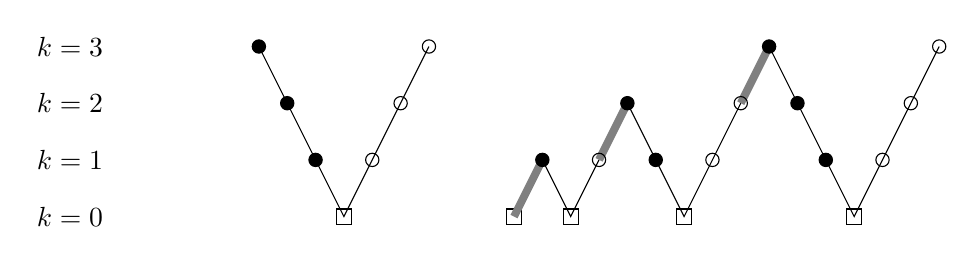
\begin{tikzpicture}[scale=1.2]
  \pgfmathsetmacro\hstep{0.3}
  \pgfmathsetmacro\vstep{0.6}
  \pgfmathsetmacro\ceps{0.08}   % size of square for coarse grid

% grid labels at left
  \node at (-2,3*\vstep) {$k=3$};
  \node at (-2,2*\vstep) {$k=2$};
  \node at (-2,\vstep) {$k=1$};
  \node at (-2,0.0) {$k=0$};

% V-cycle
  \draw[black,thin] (0.0,3*\vstep) -- (\hstep,2*\vstep) --  (2*\hstep,\vstep) -- (3*\hstep,0.0)
                    -- (4*\hstep,\vstep) -- (5*\hstep,2*\vstep) -- (6*\hstep,3*\vstep);
  \filldraw (0.0,3*\vstep) circle (2.0pt);
  \filldraw (\hstep,2*\vstep) circle (2.0pt);
  \filldraw (2*\hstep,\vstep) circle (2.0pt);
  \draw     (3*\hstep-\ceps,-\ceps) rectangle (3*\hstep+\ceps,+\ceps);
  \draw     (4*\hstep,\vstep) circle (2.0pt);
  \draw     (5*\hstep,2*\vstep) circle (2.0pt);
  \draw     (6*\hstep,3*\vstep) circle (2.0pt);

% initial coarse solve
  \pgfmathsetmacro\hoff{9*\hstep}
  \draw[shift={(\hoff,0)}]     (-\ceps,-\ceps) rectangle (+\ceps,+\ceps);
  \draw[line width=1mm,gray,shift={(\hoff,0)}] (0.0,0.0) -- (\hstep,\vstep);

% V-cycle to level 1
  \pgfmathsetmacro\hoff{10*\hstep}
  \draw[shift={(\hoff,0)},black,thin] (0.0,\vstep) -- (\hstep,0.0) -- (2*\hstep,\vstep);
  \draw[line width=1mm,gray,shift={(\hoff,0)}] (2*\hstep,\vstep) -- (3*\hstep,2*\vstep);
  \filldraw[shift={(\hoff,0)}] (0.0,\vstep) circle (2.0pt);
  \draw[shift={(\hoff,0)}]     (\hstep-\ceps,-\ceps) rectangle (\hstep+\ceps,+\ceps);
  \draw[shift={(\hoff,0)}]     (2*\hstep,\vstep) circle (2.0pt);

% V-cycle to level 2
  \pgfmathsetmacro\hoff{13*\hstep}
  \draw[shift={(\hoff,0)},black,thin] (0.0,2*\vstep) --  (\hstep,\vstep) -- (2*\hstep,0.0) -- (3*\hstep,\vstep) -- (4*\hstep,2*\vstep);
  \draw[line width=1mm,gray,shift={(\hoff,0)}] (4*\hstep,2*\vstep) -- (5*\hstep,3*\vstep);
  \filldraw[shift={(\hoff,0)}] (0.0,2*\vstep) circle (2.0pt);
  \filldraw[shift={(\hoff,0)}] (\hstep,\vstep) circle (2.0pt);
  \draw[shift={(\hoff,0)}]     (2*\hstep-\ceps,-\ceps) rectangle (2*\hstep+\ceps,+\ceps);
  \draw[shift={(\hoff,0)}]     (3*\hstep,\vstep) circle (2.0pt);
  \draw[shift={(\hoff,0)}]     (4*\hstep,2*\vstep) circle (2.0pt);

% V-cycle to finest (level 3)
  \pgfmathsetmacro\hoff{18*\hstep}
  \draw[shift={(\hoff,0)},black,thin] (0.0,3*\vstep) -- (\hstep,2*\vstep) --  (2*\hstep,\vstep) -- (3*\hstep,0.0)
                    -- (4*\hstep,\vstep) -- (5*\hstep,2*\vstep) -- (6*\hstep,3*\vstep);
  \filldraw[shift={(\hoff,0)}] (0.0,3*\vstep) circle (2.0pt);
  \filldraw[shift={(\hoff,0)}] (\hstep,2*\vstep) circle (2.0pt);
  \filldraw[shift={(\hoff,0)}] (2*\hstep,\vstep) circle (2.0pt);
  \draw[shift={(\hoff,0)}]     (3*\hstep-\ceps,-\ceps) rectangle (3*\hstep+\ceps,+\ceps);
  \draw[shift={(\hoff,0)}]     (4*\hstep,\vstep) circle (2.0pt);
  \draw[shift={(\hoff,0)}]     (5*\hstep,2*\vstep) circle (2.0pt);
  \draw[shift={(\hoff,0)}]     (6*\hstep,3*\vstep) circle (2.0pt);
\end{tikzpicture}

\caption{An FAS V-cycle (left) and F-cycle (right) on a mesh hierarchy with four levels ($K=3$).  Solid dots are \texttt{down} sweeps of NGS, open circles are \texttt{up} sweeps, and squares are \textsc{coarsesolve}. Thick grey edges show $\hat P$.}
\label{fig:cycles}
\end{figure}

V-cycles can be iterated to solve problem \eqref{feweakform} to desired accuracy.  We put this in a pseudocode for clarity:
\begin{pseudo*}
\pr{fas-solver}(w^K,\id{rtol}=10^{-4},\id{cyclemax}=100)\text{:} \\+
    $\ell^K[v] = \ip{g}{v}$ \\
    $r_0 = \|\ell^K - F^K(w^K)\|$ \\
    for $s=1,\dots,\id{cyclemax}$ \\+
        \pr{fas-vcycle}(K,w^K,\ell^K) \\
        if $\|\ell^K-F^K(w^K)\| < \id{rtol}\,r_0$ \\+
            break \\--
    return $w^K$
\end{pseudo*}

Our Python code \texttt{fas1.py} implements \pr{fas-vcycle} and \pr{fas-solver}, and options \texttt{-rtol}, \texttt{-cyclemax} override the defaults for the latter.  As is easily seen by experimentation, and as we will demonstrate in the next two sections, 7 to 12 V-cycles, using the default settings in \textsc{fas-vcycle} including \texttt{down} $=1$ and \texttt{up} $=1$ smoother applications, make a very effective solver on any mesh.

But we can add a different multilevel idea to get a new kind of cycle.  It is based on the observation that an iterative equation solver, linear or nonlinear, often depends critically on the quality of its initial iterate.  Indeed, choosing initial iterate $w^K=0$ and calling \textsc{fas-solver} may not yield a convergent method.  However, one finds in practice that coarse meshes are more forgiving with respect to the initial iterate than are finer meshes.  Now the new idea is to start on the coarsest mesh in the hierarchy, where a blind guess like $w^0=0$ is most likely to succeed, and then work upward through the levels.  At each mesh level one computes an initial iterate by prolongation of a nearly-converged iterate on the previous level, and then one does a V-cycle.  At the finest mesh level we may do repeated V-cycles.

The resulting algorithm is called an FAS multigrid ``F-cycle'' because the pattern in Figure \ref{fig:cycles} (right) looks vaguely like an ``F'' on its back; it is the following algorithm:
\begin{pseudo*}
\pr{fas-fcycle}(K,\id{down}=1,\id{up}=1)\text{:} \\+
    $w^0 = 0$ \\
    $\ell^0[v] = \ip{g}{v}$ \\
    \pr{coarsesolve}(w^0,\ell^0) \\
    for $k=1,\dots,K$ \\+
        $w^k = \hat P w^{k-1}$ \\
        $\ell^k[v] = \ip{g}{v}$ \\
        \pr{fas-vcycle}(k,w^k,\ell^k) \\-
    return $w^K$
\end{pseudo*}
Note that parameters \id{down} and \id{up} are passed into the V-cycle.

This algorithm is also called a ``full multigrid'' (FMG) cycle \cite{BrandtLivne2011,Briggsetal2000}, but the meaning of ``full'' is fundamentally different in FAS versus FMG terminology.  One may run \pr{fas-fcycle} to generate the initial iterate for \pr{fas-solver}, as as we will see in section \ref{sec:performance}, the result of one F-cycle is already a very good solution.

It is important to avoid the introduction of high frequencies as one generates the first iterate on the finer mesh.  Thus a coarse-mesh solution is prolonged on to the next level by a possibly-different operator:
\begin{equation}
  w^k = \hat P w^{k-1} \label{enhancedprolongation}
\end{equation}
It is common for a better interpolation scheme to be used for $\hat P$ than for $P$ \cite{Trottenbergetal2001}.  Our choice for $\hat P$ first applies $P$ to generate a fine-mesh function, but followed by sweeping once through the \emph{new} fine-mesh nodes and applying NGS there without altering values at the nodes already present in the coarse mesh.  This $\hat P$ is half of a smoother, and counted as such; see section \ref{sec:performance}.


\section{Convergence} \label{sec:convergence}

The Python program \texttt{fas1.py} accompanying this note applies \pr{fas-solver} by default, with zero initial iterate, to solve equation \eqref{liouvillebratu}.  The program depends only on the widely-available NumPy library \cite{Harrisetal2020}.  It imports local modules \texttt{meshlevel.py}, \texttt{problems.py}, and \texttt{cycles.py} from the same directory.

To get started, clone the Git repository and run the program:
\begin{cline}
$ git clone https://github.com/bueler/mg-glaciers.git
$ cd mg-glaciers/fas/py/
$ ./fas1.py
  m=8 mesh, 6 V(1,1) cycles (19.50 WU): |u|_2=0.102443
\end{cline}
%$
Various allowed options to \texttt{fas1.py} are shown by usage help:\footnote{Also, a small suite of software (regression) tests of \texttt{fas1.py} is run with \,\texttt{make test}.}
\begin{cline}
$ ./fas1.py -h
\end{cline}
%$
For example, choosing a mesh with $m=2^{K+1}=16$ elements and a problem with known exact solution (section \ref{sec:intro}), yields Figure \ref{fig:show}:
\begin{cline}
$ ./fas1.py -K 3 -mms -show
  m=16 mesh, 6 V(1,1) cycles (21.75 WU): ... |u-u_ex|_2=2.1315e-02
\end{cline}
%$
The V-cycles in this run, exactly as shown in Figure \ref{fig:cycles}, are reported as ``\texttt{V(1,1)}'' because the defaults correspond to \texttt{down} $=1$ and \texttt{up} $=1$ NGS sweeps on each level.  Note that runs with option \texttt{-mms} report the final numerical error $\|w^h-u\|_2$.

\begin{figure}
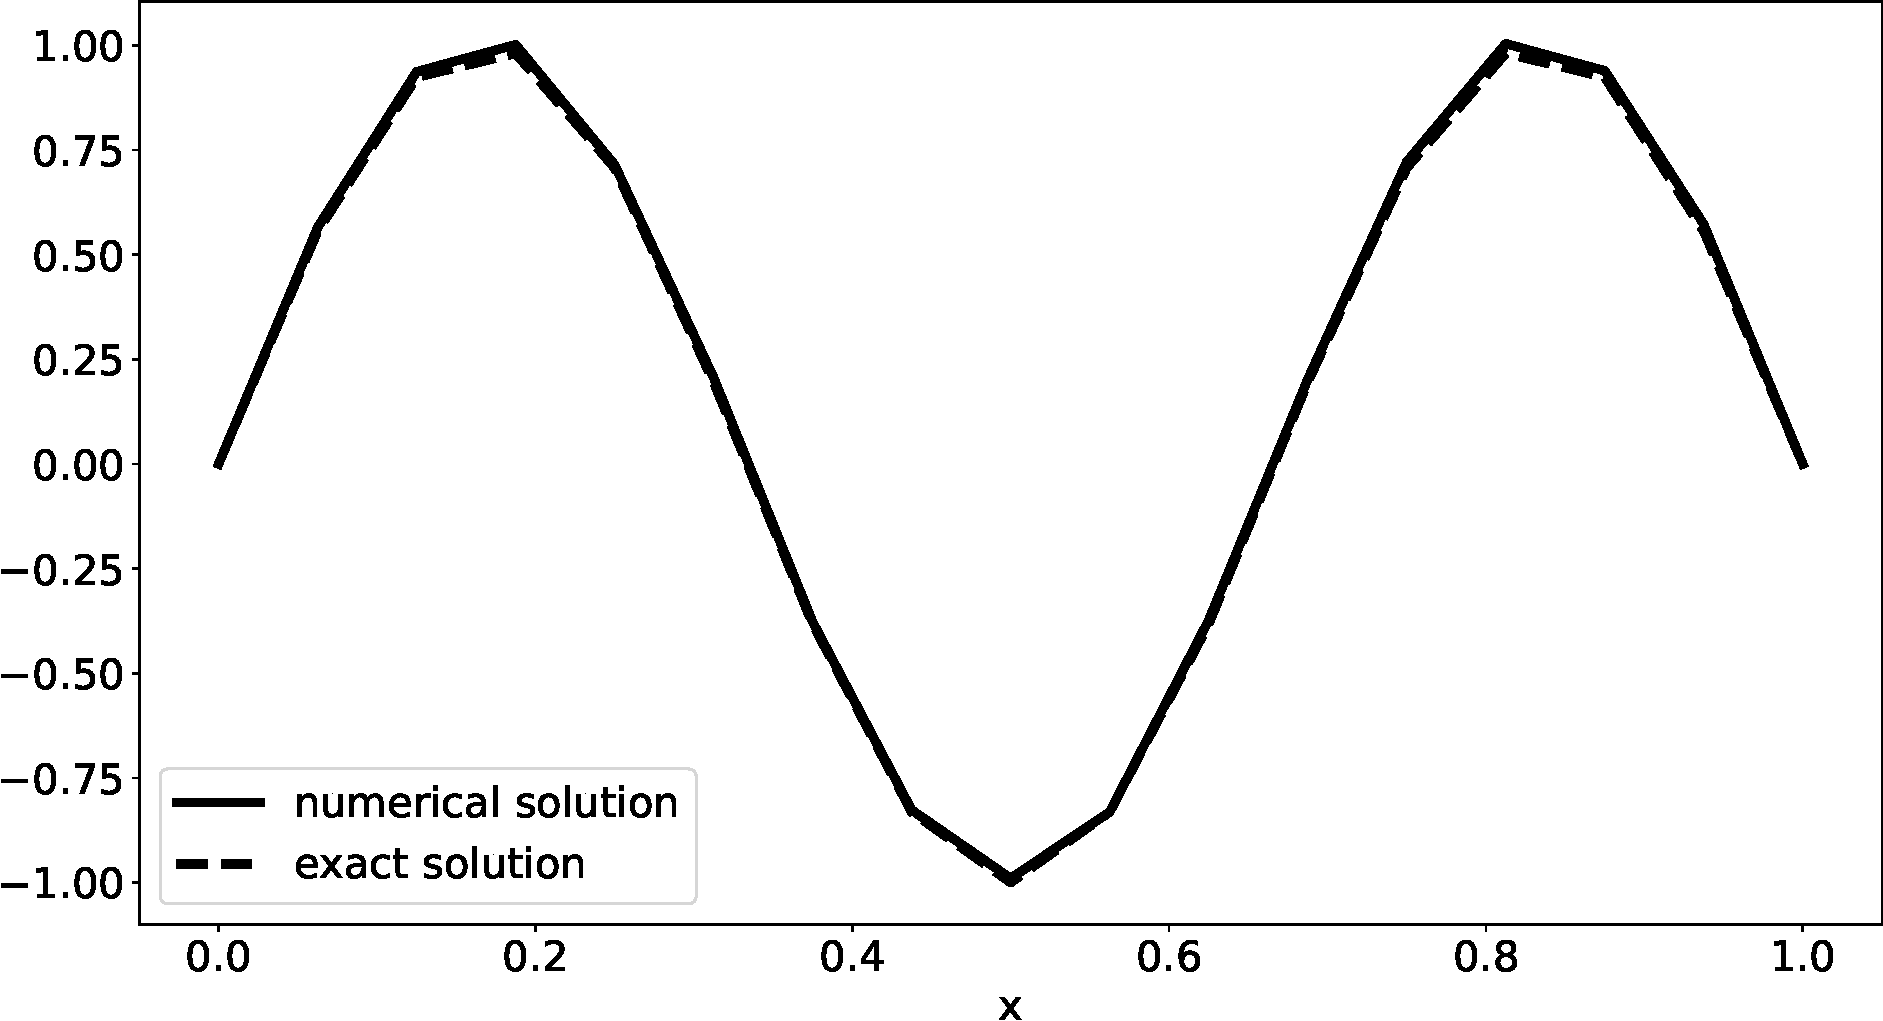
\includegraphics[width=0.8\textwidth]{figs/show.pdf}
\caption{Results from a \texttt{-mms} run of \texttt{fas1.py} on $m=16$ elements.}
\label{fig:show}
\end{figure}

By using the \texttt{-mms} case we can demonstrate convergence of our implemented FE method, and thereby verify \texttt{fas1.py}.  The numerical error from runs with 12 V-cycles, i.e.~with options \texttt{-rtol 0 -cyclemax 12}, and $K=3,4,\dots,14$ corresponding to $16\le m \le 32768$ elements, are shown in Figure \ref{fig:converge}.  Because our problem is so simple, with a very smooth solution, the convergence rate is exactly at the expected rate $O(h^2)$ \cite{Elmanetal2014}.

However, if instead of a small, fixed number of V-cycles we instead try a large number of NGS sweeps, e.g.~we apply the algorithm below with \texttt{-rtol 0 -cyclemax 10000} and zero initial iterate, then the results are disappointing.
\begin{pseudo*}
\pr{ngsonly}(w^K,\id{rtol}=10^{-4},\id{cyclemax}=100)\text{:} \\+
    $\ell^K[v] = \ip{g}{v}$ \\
    $r_0 = \|\ell^K - F^K(w^K)\|$ \\
    for $s=1,\dots,\id{cyclemax}$ \\+
        \pr{ngssweep}(w^K,\ell^K) \\
        if $\|\ell^K-F^K(w^K)\| < \id{rtol}\,r_0$ \\+
            break \\--
    return $w^K$
\end{pseudo*}
As shown in Figure \ref{fig:converge}, such runs generates convergence to discretization error only on meshes with $m=16,32,64,128$.  For slightly finer meshes ($m=256,512$) the same number of sweeps is no longer sufficient, and continuing to yet finer meshes using the same number of sweeps would make essentially no progress (not shown).  The reason for this behavior is that almost all of the algebraic error (section \ref{sec:femethod}) is in low-frequency modes which the NGS sweeps are barely able to reduce.  This is the situation which multigrid schemes are designed to address \cite{BrandtLivne2011,Briggsetal2000}: by moving the problem between meshes the same smoother will efficiently-reduce all frequencies present in the error.  Both the smoother and the coarse-level solver components of our FAS algorithms consist entirely of NGS sweeps, but by adding a multilevel mesh infrastructure we have arranged that the sweeps are always making progress.

\begin{figure}
\includegraphics[width=0.7\textwidth]{figs/converge.pdf}
\caption{For a fixed number of V-cycles the numerical error $\|u-u_{\text{ex}}\|_2$ converges to zero at the expected rate $O(h^2)$.  Even $10^4$ NGS sweeps fail to converge at higher resolutions.}
\label{fig:converge}
\end{figure}


\section{Performance}  \label{sec:performance}

Having verified our method, our first performance test compares three solver algorithms:
\begin{itemize}
\item \textsc{fas-fcycle}, defined in section \ref{sec:cycles}.
\item \textsc{fas-solver}, which does V-cycles, defined in section \ref{sec:cycles}.
\item \textsc{ngsonly}, defined in section \ref{sec:convergence}.
\end{itemize}
The two FAS algorithms actually represent many different algorithms according to the different options.  While making no attempt to systematically-explore the parameter space, we observe that 7 to 12 V(1,1) cycles suffice to approach discretization error in the \texttt{-mms} problem.  For F-cycles we must choose how many V-cycles to take once the finest level is reached, and 2 or 3 certainly suffice.  Experimentation in minimizing the work units (below), while maintaining convergence, yields a choice of three V(1,0) cycles.

The three chosen algorithms become the following specific \texttt{fas1.py} options on meshes with $m=2^{K+1}$ elements for $K=3,4,\dots,17,18$:

\medskip
\begin{tabular}{ll}
\textsf{F-cycle$+$3$\times$V(1,0)} \,:        &\texttt{-mms -fcycle -rtol 0 -cyclemax 4 -up 0 -K }$K$ \\
\textsf{12 V(1,1) cycles} \,:  &\texttt{-mms -rtol 0 -cyclemax 12 -K }$K$ \\
\textsf{NGS sweeps} \,:      &\texttt{-mms -rtol 0 -cyclemax $Z$ -ngsonly -K }$K$
\end{tabular}

\medskip
In order to achieve convergence for NGS sweeps alone, we must choose rapidly increasing $Z$ as $K$ increases.  For the comparison below we simply double $Z$ until the reported numerical error is within a factor of two of discretization error (as reported by the FAS algorithms), but at $K=7$ the time is 100 seconds and we stop testing.

The results for run time on the author's laptop are in Figure \ref{fig:optimal}.  For all the coarser meshes, e.g.~$m=16,\dots,256$, the FAS algorithms run in about 0.3 seconds.  This is the minimum time to start and run any Python program on this machine, so the actual computational time is not really detected.  For $m \ge 10^3$ both FAS algorithms enter into a regime where the run time is greater than one second, and then it becomes proportional to $m$.  That is, their solver complexity is $O(m^1)$.  These are \emph{optimal} solvers \cite[Chapter 7]{Bueler2021}.

By contrast, the \pr{ngsonly} algorithm is far from optimal, and not capable of solving on fine meshes.  Fitting the three finest-mesh completed cases suggests its time is $O(m^{3.5})$.

\begin{figure}
\includegraphics[width=0.7\textwidth]{figs/optimal.pdf}
\caption{Run time to reach discretization error is optimal $O(m)$ for both V-cycles and F-cycles.  Run time explodes for NGS sweeps.}
\label{fig:optimal}
\end{figure}

A standard way to compare multigrid-type solver algorithms uses the concept of a \emph{work unit} (WU).  One WU is the number of operations needed to do one smoother sweep on the finest mesh, which takes $O(m)$ arithmetic (floating point) operations.  For WUs in a 1D multilevel scheme, note that a smoother sweep on the second-finest mesh is $\frac{1}{2}$WU, and so on downward in the hierarchy, so the total of WU for a multigrid algorithm is a finite geometric sum \cite{Briggsetal2000} which depends on the number of levels $K$.  For simplicity we do not count the arithmetic work in restriction and prolongation, other than in the enhanced prolongation $\hat P$ in \eqref{enhancedprolongation}, which uses $\frac{1}{2}$WU when passing to the finest mesh.  Also we ignore non-arithmetic work entirely, for example vector copies.

Consider the $K\to\infty$ limit of WU calculations for the three algorithms above:
\begin{align*}
\text{WU}\big(\text{\textsf{F-cycle$+Z\times$V(1,0)}}\big) &\approx 3+2Z \\
\text{WU}\big(\text{\textsf{$Z$ V(1,1) cycles}}\big)   &\approx 4Z \\
\text{WU}\big(\text{\textsf{$Z$ NGS sweeps}}\big)      &= Z
\end{align*}
(Note that counting work units for NGS sweeps is trivial.)  To confirm this we have added WU counting to \texttt{fas1.py}.  On a $K=10$ mesh with $m=2^{11}=2048$ elements, for example, we observe that \textsf{F-cycles$+$3$\times$V(1,0)} requires a measured 8.98 WU while \textsf{12 V(1,1) cycles} uses 47.96 WU.

In fact a single F-cycle, without any additional V-cycles, nearly reaches discretization error.  Consider three single-F-cycle schemes.  The first is ``F(1,1)'', which uses the default settings \id{down}=1 and \id{up}=1.  The other two are ``F(1,0)'', using \id{up}=0, and ``F(1,0)+$\Rin$'', which changes from the default full-weighting restriction ($\Rfw$) to injection ($\Rin$).  These three solvers use 9, 5, and 5 WU, respectively, in the $K\to\infty$ limit of many levels.  The Figure shows that on $K=7,\dots,18$ meshes, with up to $m=2^{19} = 5 \times 10^5$ elements, the measured numerical error is within a factor of two of discretization error.  Note that the down-smoother-only F-cycles actually generate smaller errors.  On the finest mesh it seems the discretization error itself, of order $10^{-11}$, was corrupted by rounding errors, and so all the measured numerical errors are closer together.  Some multigrid authors \cite[for example]{BrownSmithAhmadia2013} use ``textbook multigrid efficiency'' to mean ``less than 10 WU to achieve discretization error'', and by that standard our F-cycles exhibit textbook multigrid efficiency.

\begin{figure}
\includegraphics[width=0.7\textwidth]{figs/tme.pdf}
\caption{Computed numerical error, relative to discretization error, from three versions of a single F-cycle.}
\label{fig:tme}
\end{figure}


\section{Extensions}  \label{sec:extensions}

Our program \texttt{fas1.py} is deliberately basic in many senses.  Here are four possible extensions which the reader might want to implement, roughly ordered from easiest to most difficult:
\renewcommand{\labelenumi}{\textbf{\Roman{enumi}.}}
\begin{enumerate}
\item The number of V-cycles, either in simple iterative usage or as the finest-level action in an F-cycle, is fixed by the option \texttt{-cycles}.  It would be natural to instead use relative and absolute residual norm tolerances as stopping criteria.  For example, one might set \texttt{rtol} and \texttt{atol} so that V-cycles stop when either of the following conditions hold for the $j$th iterate $w^j$ on the finest mesh:
    $$\frac{\|r^K(w^j)\|_2}{\|r^K(w^0)\|_2} \le \text{\texttt{rtol}} \quad \text{or} \quad \|r^K(w^j)\|_2 \le \text{\texttt{atol}}.$$
Example default values are \texttt{rtol} $=10^{-8}$ and \texttt{atol} $=10^{-50}$ \cite{Bueler2021}.
\item The default value of the parameter $\lambda$ in \eqref{liouvillebratu} is \texttt{-lam 1.0}, but one can check that the $g=0$ problem becomes unstable at a critical value $\lambda_c \approx 3.5$.  Interestingly, the solution changes very little as $\lambda \nearrow \lambda_c$; things are boring until failure occurs.  (The most-common numerical symptom is overflow of $e^u$.)  Equation \eqref{liouvillebratu} is a very simple model for combustion of a chemical mixture, and this instability corresponds to a chemical explosion \cite{FrankKameneckij1955}.  However, finding $\lambda_c$ precisely is not easy because \texttt{fas1.py} always initializes at the distant location $w^0=0$.  The behavior of FAS F-cycles is especially nontrivial near the critical $\lambda$ because the critical value is different on coarse grids.  (And apparently sometimes smaller!)  A better strategy for solutions near the critical value, and for parameter studies generally, is ``continuation''.  For example, one might use a saved fine-mesh solution as the initial value in a run with a slightly-different $\lambda$ value.  The new run would then only need a few V-cycles.
\item Equation \eqref{liouvillebratu} is a ``semilinear'' ODE because the nonlinearity occurs in the zeroth-derivative term \cite{Evans2010}.  One might instead solve a ``quasilinear'' equation where the nonlinearity is in the coefficient to the highest-order derivative.  For example, one might try a $p$-Laplacian \cite{Evans2010} extension to the Liouville-Bratu equation:
\begin{equation}
  -\left(|u'|^{p-2} u'\right)' - \lambda e^u = g.  \label{pbratu}
\end{equation}
This equation is the same as \eqref{liouvillebratu} when $p=2$, but for other values $p$ in $(1,\infty)$ the solution is less well-behaved because the coefficient of $u''$ can degenerate or explode.  However, a literature at least exists for the corresponding Poisson problem ($\lambda=0$) \cite{BarrettLiu1993,Bueler2021,Evans2007}.  A basic technique is to regularize the leading coefficient with a numerical parameter $\eps>0$: replace $|u'|^{p-2}$ with $\left(|u'|^2+\eps\right)^{(p-2)/2}$.  With such a change, continuation (item \textbf{II}) will be both important and a bit complicated.
\item By far the most consequential extension of \texttt{fas1.py} would be to ``merely'' change from 1D to 2D or 3D.  That is, to change from solving ODEs to solving elliptic PDEs like $-\grad^2 u - \lambda e^u=g$, where $\grad^2$ is the Laplacian operator.  However, doing this in the style of \texttt{fas1.py}, using only NumPy vectors for infrastructure, is not recommended.  Instead, application of a finite element library like Firedrake \cite{Bueler2021,Rathgeberetal2016} or Fenics \cite{Loggetal2012} would be wise.  Using such libraries requires a substantial learning curve, and these libraries do not have full support for FAS multigrid methods, but using such libraries would also allow experimentation with higher-order finite element spaces and many other benefits.
\end{enumerate}


\section{Conclusion}  \label{sec:conclusion}

Regarding the performance of the three solvers listed in the last section, we summarize as follows:

\begin{quotation}
\emph{On any mesh of practical effective resolution, say with $m>10^2$ elements, problem \eqref{feweakform} can be solved to within the discretization error of our piecewise-linear FE method by using \textsc{fas-f}$(3)$ or \textsc{fas-vcycles}$(12)$.  This holds for all $m$, up to values where rounding error overwhelms the discretization error, at around $m=10^6$.  By contrast, for \textsc{ngsonly}$(Z)$ we must increase $Z$ rapidly with $m$; for example $Z > 10^3$ is required if $m>10^2$.  If $m>10^3$ then discretization error cannot be achieved by \textsc{ngsonly}$(Z)$ in reasonable time.}
\end{quotation}

In other words, the two FAS methods require only a small number of cycles $Z$, independently of the mesh resolution.  When we measure the computational work required for the three algorithms we see that the amount of work is proportional to $mZ$ in all cases, but both FAS methods are optimal solvers which require only $O(m)$ work because $Z$ can be fixed.  The faster F-cycle gives textbook multigrid efficiency.


\small

\bigskip
\bibliography{fas}
\bibliographystyle{siam}

\end{document}
